\section{Diagrama de Classes}

Nesta secção, apresentamos, na figura \ref{fig:diagrama_de_classes}, o diagrama de classes da nossa aplicação.


Nele estão representadas as classes que fazem parte do package \emph{Funcionalidade}(fig. \ref{fig:diagrama_de_packages}), as quais consistem nas classes de acesso à base de dados, como \emph{AConnection} e os vários \emph{DAO}s e as restantes classes que definem as entidades.


\begin{figure}[h]
    \centering
    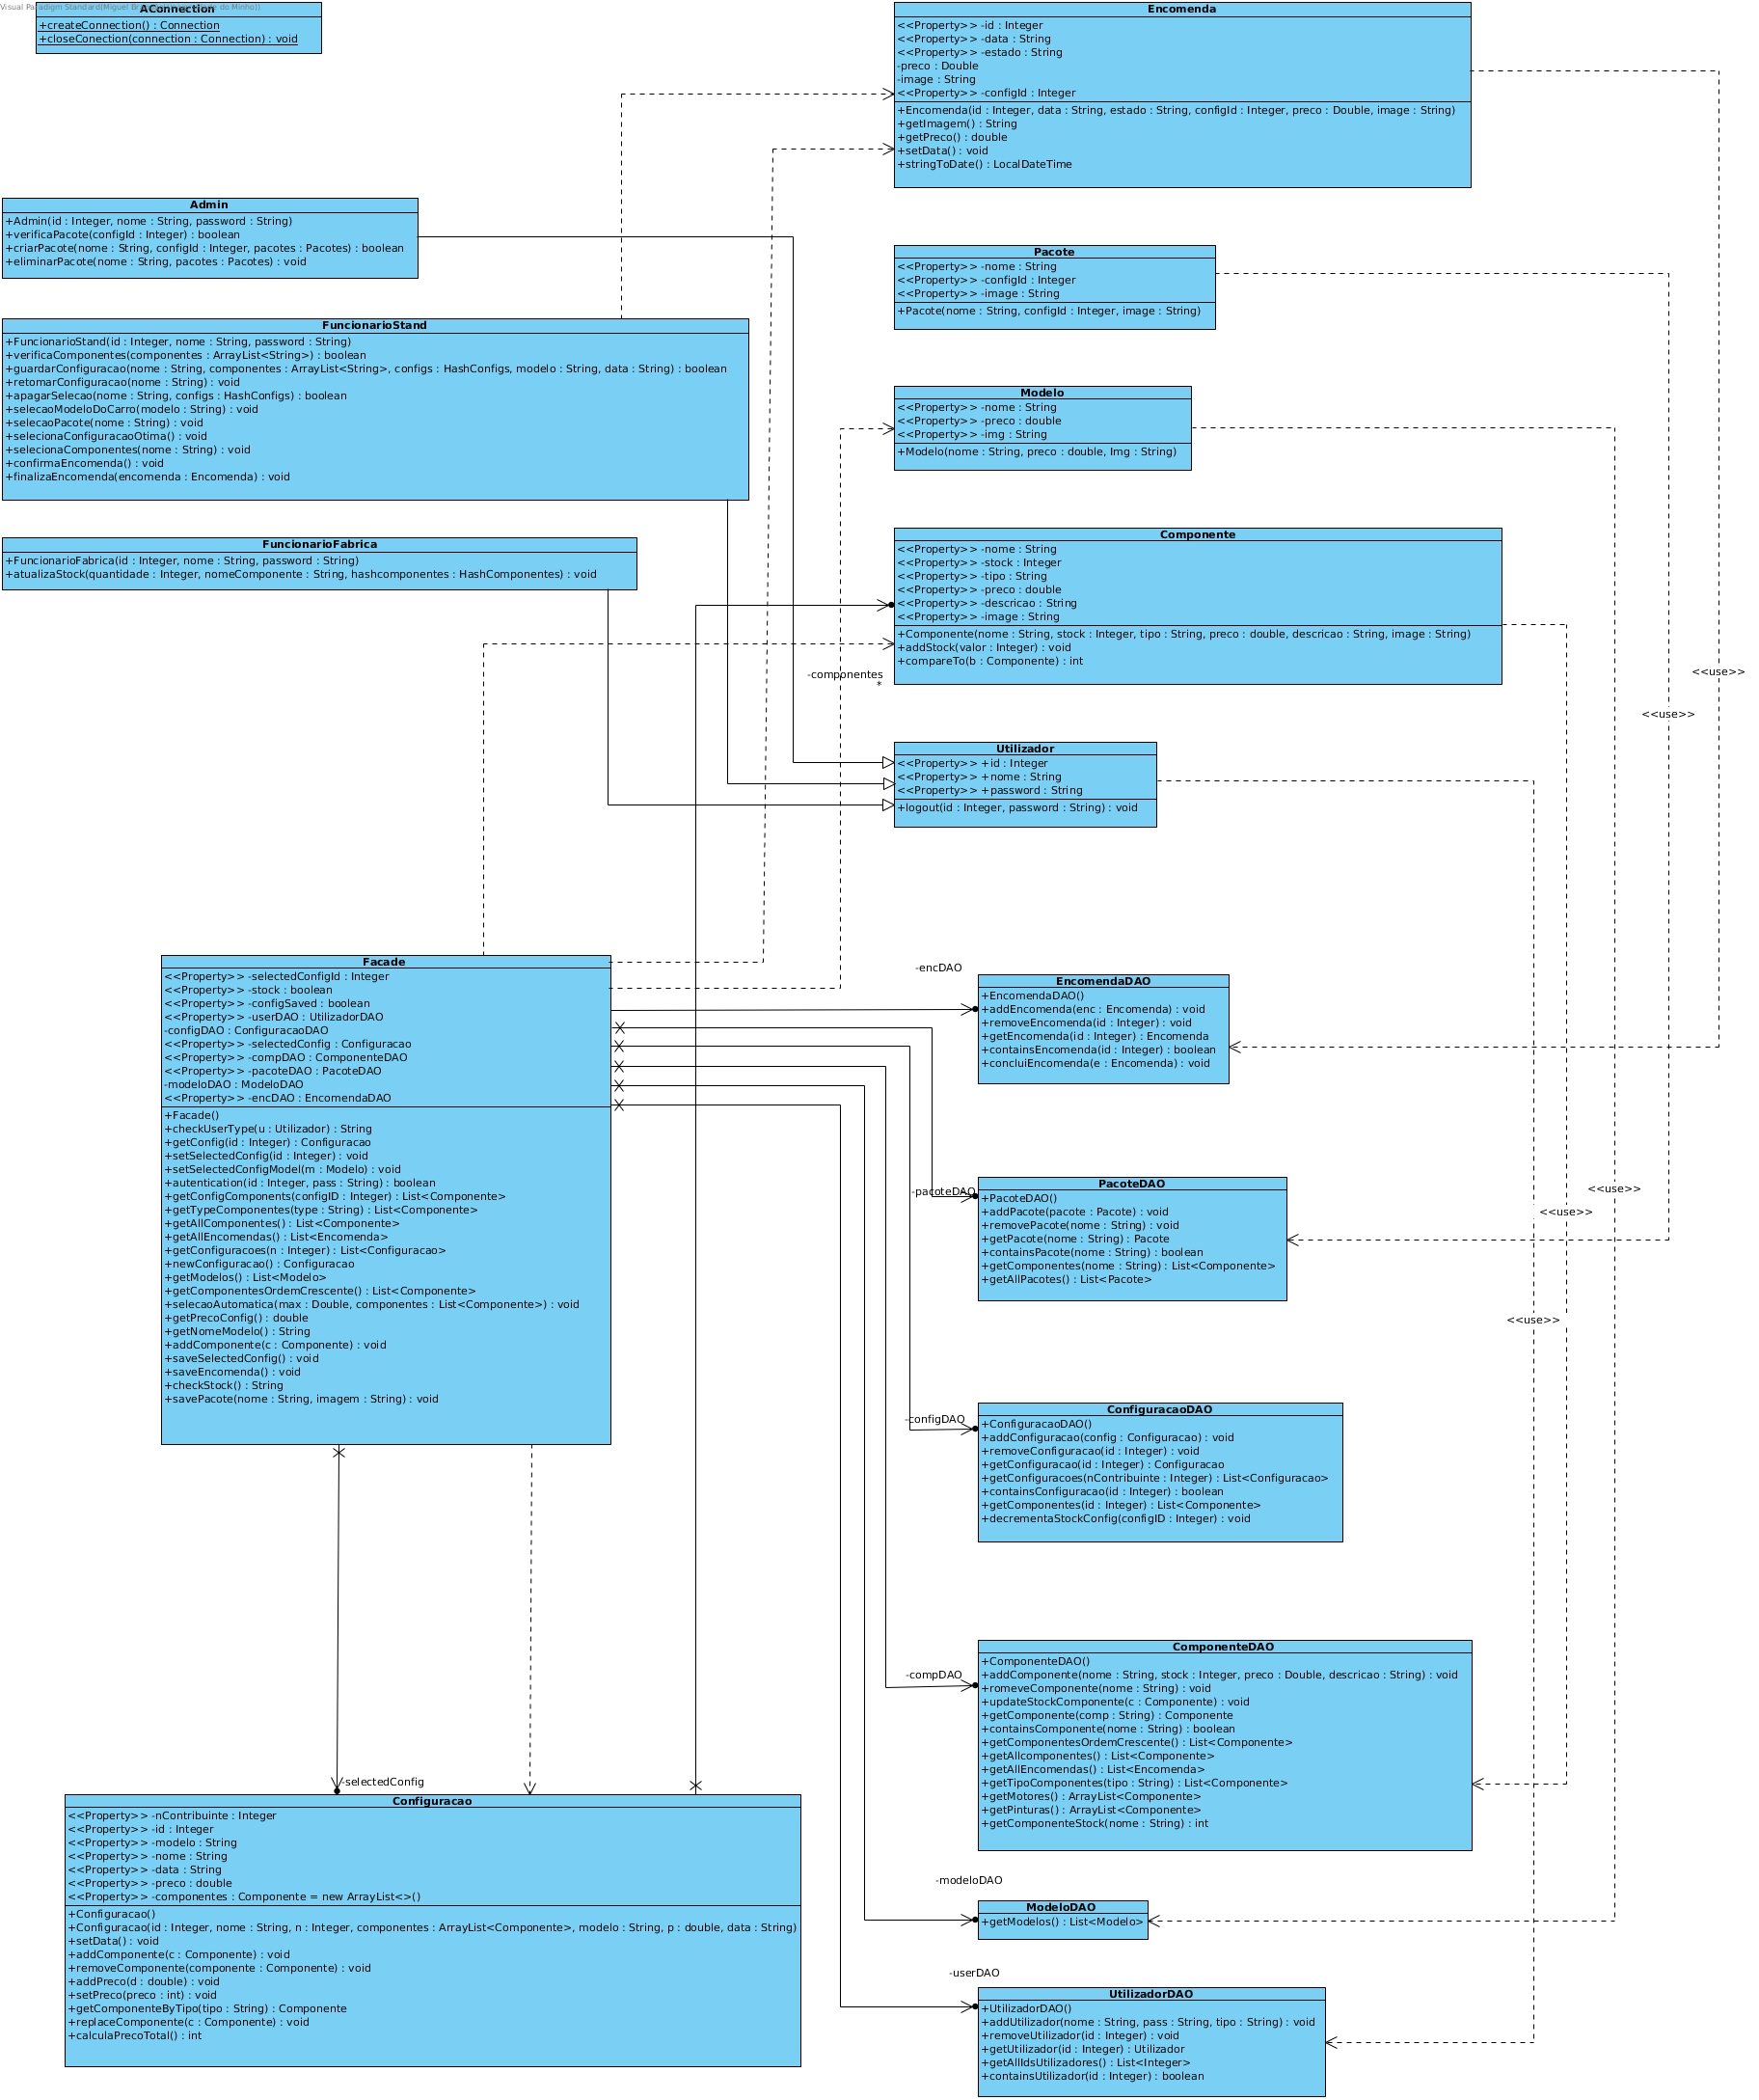
\includegraphics[width=\textwidth]{diagrama_de_classes/diagrama_de_classes.jpg}
    \caption{Diagrama de classes}
    \label{fig:diagrama_de_classes}
\end{figure}

\section{Diagrama de packages}

Nesta secção, apresentamos, na figura \ref{fig:diagrama_de_packages}, o diagrama de packages da nossa aplicação.

Neste diagrama, estão representados os dois packages que decidimos criar. O package \emph{Funcionalidade} contém todas as classes de controlo do programa, enquanto que o package \emph{InterfaceGrafica}, tal como o nome indica, contém todas as classes que fazem a interface gráfica. 

\begin{figure}
    \centering
    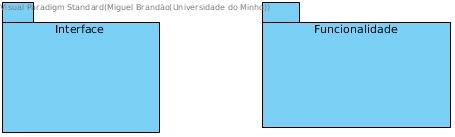
\includegraphics[width=\textwidth]{diagrama_de_classes/diagrama_de_packages.jpg}
    \caption{Diagrama de packages}
    \label{fig:diagrama_de_packages}
\end{figure}
